\documentclass[man]{apa7}

% Referencing Packages
\usepackage[english]{babel}
\usepackage{csquotes}
\usepackage[style=apa,sortcites=true,sorting=nyt,backend=biber]{biblatex}
\DeclareLanguageMapping{english}{english-apa}
\addbibresource{study1.bib}

% Other Packages
\usepackage{orcidlink}
\usepackage{geometry}
\usepackage{graphicx}
\usepackage{txfonts}
\usepackage{hyperref}
\usepackage{hypernat}
\usepackage{url}
\usepackage{enumitem}
\usepackage{xspace}
\usepackage{float}
\usepackage{rotating, lscape, nicematrix, longtable, tabu, bookmark, booktabs, siunitx, multirow}
\usepackage{array}
\usepackage{setspace}
\usepackage[utf8]{inputenc}
\usepackage{textgreek}
\usepackage{endnotes}
\usepackage[font=normal, skip=0pt]{caption}
\usepackage{subcaption}

% Tables and Figures path
\graphicspath{{./tables_and_figs/figs/}}

% Make new column types
% Top align
\newcolumntype{C}[1]{>{\centering\let\newline\\\arraybackslash\setstretch{1.0}}p{#1\columnwidth}}
\newcolumntype{L}[1]{>{\raggedright\let\newline\\\arraybackslash\setstretch{1.0}}p{#1\columnwidth}}
\newcolumntype{R}[1]{>{\raggedleft\let\newline\\\arraybackslash\setstretch{1.0}}p{#1\columnwidth}}
% Bottom align
\newcolumntype{S}[1]{>{\centering\let\newline\\\arraybackslash\setstretch{1.0}}b{#1\columnwidth}}
\newcolumntype{A}[1]{>{\raggedright\let\newline\\\arraybackslash\setstretch{1.0}}b{#1\columnwidth}}
\newcolumntype{D}[1]{>{\raggedleft\let\newline\\\arraybackslash\setstretch{1.0}}b{#1\columnwidth}}

% Title Page
\title{Bias in Candidate Sourcing Communication:\\Investigating Stereotypical Gender- And Age-Related Frames in Online Job Advertisements at the Sectoral Level}
\shorttitle{Bias in Candidate Sourcing Communication}

\authorsnames[1,1,{2},1,{3}]{Noon M.F. Abdulqadir, Anne Kroon, Martine van Selm, Margot van der Goot, and Rens Vliegenthart}
\authorsaffiliations{
    {Amsterdam School of Communication Research (ASCoR)},
    {Erasmus School of History, Culture and Communication (ESHCC)},
    {Wageningen University and Research (WUR)}
}

\leftheader{Noon et al.}

\abstract{Studies show the extent to which job advertisements contain stereotypical wordings correlates with the level of segregation at individual job level and boarder occupation level. However, limited research links the framing of job ads to gender- and age-based segregation at the sector level. Guided by the stereotype content model, we operationalize stereotypical warmth and competence-related frames in candidate sourcing communication and investigate their presence in job ads from occupational sectors with varying levels of segregation. Automated content analysis was conducted on a dataset of online job ad sentences (\textit{n}=307154). Results indicate warmth-related frames are most observed in ads from female-dominated (vs. male-dominated) and younger-dominated (vs. older-dominated and mixed-age) dominated sectors. Conversely, competence-related frames are most observed in ads from male-dominated (vs. female-dominated and mixed-gender) and older-dominated (vs. younger-dominated and mixed-age) sectors. Taken together, we present an operationalization of stereotypical warmth- and competence-related frames in early employer communication and posit that social categorization framing may be at play.}

\keywords{automated content analysis, occupational segregation, social categorization frames, stereotype content model}

\authornote{
   \addORCIDlink{Noon M.F. Abdulqadir}{https://orcid.org/0000-0002-6243-9241}

   \addORCIDlink{Anne Kroon}{https://orcid.org/0000-0001-7600-7979}

   \addORCIDlink{Martine van Selm}{https://orcid.org/0000-0001-9188-4021}

   \addORCIDlink{Margot van der Goot}{https://orcid.org/0000-0001-6904-6515}

   \addORCIDlink{Rens Vliegenthart}{https://orcid.org/0000-0003-2401-2914}

   \qquad We have no conflicts of interests to disclose.

   \qquad Correspondence concerning this article should be addressed to Noon Abdulqadir, Postbus 15791, 1001 NG Amsterdam. Email: noon.abdulqadir@uva.nl

   \qquad \textbf{Suggested citation:} Noon, M. A., Kroon, A. C., van Selm, M., van der Goot, M., and Vliegenthart, R. (2021). Bias in Candidate Sourcing Communication: Investigating Stereotypical Gender- and Age-Related Frames of Online Job Advertisements at the Sectoral Level.}

% Main Body
\begin{document}
% \maketitle
% Scholars have long documented the influence of interpersonal bias in candidate recruitment, particularly with regard to job seekers’ gender and age \parencite{beattie_possible_2012, heilman_gender_2012, paleari_when_2019}. This influence is observable during active candidate sourcing where job advertisements represent the first touchpoint in employer communication \parencite{RynesS.1989}. These job ads can signal essential value-related information about an organization \parencite{de_cooman_portraying_2012} but can also determine the pool of potential candidates who apply for an advertised position and reinforce existing interpersonal biases. On the micro-level, job ads and the HR decisions that dictate their content are informed by the type of candidate employers explicitly or implicitly envision as “ideal” for a position \parencite{kelly_gendered_2010}. \Textcite{van_selm_search_2021}, for instance, found that job ads targeting older workers contained frames consistent with general stereotypes of older individuals. On the meso-level, the content of job ads can also reflect the level of segregation (homogeneity), or lack thereof (heterogeneity), in an occupation. As \Textcite{gaucher_evidence_2011} found, job ads from traditionally male-dominated occupations such as engineer, plumber, and security guard tend to contain terms such as competitive, leader, ambitious, and similar wordings that are culturally related to masculinity, consequently making such ads less appealing to female candidates.

% Thus far, limited research has explored the relationship between the content of job advertisements and macro-level occupational segregation, i.e., at the sectoral level, demarcated specifically by social category composition \parentext{with the exception of \nptextcite{garcia-retamero_prejudice_2006} as cited in \nptextcite{clarke2020GenderStereotypesGenderTyped}}. Although career changes across sectors are more common than ones across occupations \parencite{carrillo-tudela_extent_2016}, workers generally tend to stay within social category-typed sectors due to expected backlash effect \parencite{fritsch_horizontal_2020}. For example, a female social worker making a career change from the Health and social work activities sector may be more likely to go into the Education or Government and care sectors, both highly female-dominated. Similarly, an older logistics manager in the Transportation and storage sector may more readily consider a career as a production manager in the Manufacturing sector than an ICT-manager in the younger-typed Information and communication sector. Sectoral segregation demarcated based on social category composition may thus be more persistent and present a higher social barrier to entry than segregation demarcated based on other occupational factors, thus becoming key to understanding possible inequity in candidate sourcing.

% Given this, the present study makes three main contributions. First, it investigates candidate sourcing in Dutch intranational sectors that are heterogeneous and homogenous in gender and age composition, i.e., female- and male-dominated (vs. mixed-gender sectors) and older worker- and younger worker-dominated (vs. mixed-age sectors respectively). Informed by framing theory and the stereotype content model, we examine the extent to which framed gender- and age-related stereotypes are present in online job ads from heterogeneous and homogenous sectors. Second, it presents a systematic operationalization of broad-level gender- and age-related stereotypical frames in job ads. Employing the social categorization framing hypothesis \parencite{Yang2015a}, we adopt the conceptualization of pancultural and generalizable warmth- and competence-related social category stereotypes put forth in the SCM \parencite{fiske_model_2002}. Third, we utilize a rigorous automated content analysis method that serves as an exemplary analysis of how to detect biases in texts. This study thus seeks to answer the question: \textit{to what extent are job advertisements from social category-typed occupational sectors framed in terms of warmth- and competence-based gender and age stereotypes?}

% \subsection{Framing Theory and Stereotypical Frames}
% \label{framing}
% Framing a message constrains its audiences to desired and meaningful interpretations by directing attention to information judged to be important by the message sender. Frames make salient some aspects or subset of possible considerations about a subject over others \parencite{entman_framing_1993}, typically through strategic “selection, emphasis, exclusion, and elaboration” \parencite[p. 10] {reese_framing_2001}. Within framing theory, stereotypes are a powerful framing device underscored by culturally-embedded implicit reasoning devices \parencite{van_gorp_where_2005}, i.e., they draw on and activate culturally shared (consensual) cognitive schemata. In their capacity as framing devices, stereotypes draw attention to a particular assessment of social categories, their roles, and their distance from the reader.

% Expounding on the use of stereotypes in framing, \parencite{Yang2015a} presents a typology of stereotypical frame genres differentiated through their effects on cognition and the pathway by which they make salient the perceived social distance between categories, i.e., degree of emphasis on the self-to-other differences. \textit{Social categorization frames} in particular are germane to the current study as their usage centers around ownership of cultural objects such as social roles or certain jobs and occupational sectors. By emphasizing the belongingness of cultural objects to select social categories, social categorization frames activate distinct social identities, otherization, and make salient the social distance between social categories. This frame genre thus conveys the reasoning that “certain groups are outgroups and their members are not qualified for ingroup activities” \parencite[p. 261]{Yang2015a}. Likewise, social categorization frames may activate self-stereotyping and lead to ingroup members assuming the characteristics stereotypically associated with their category, increasing conformity and deindividuation \parencite{brown2003BlackwellHandbookSocial}.

% Social categorization frames are also applied differently to different categories depending on whether they are dominant or non-dominant in a domain. When addressing dominant social categories, emphasis is placed on ingroup characteristics and their complementarity to features of the cultural object. When addressing outgroups, the information also tends to be stereotype-consistent, however, the emphasis is on the mismatch between the cultural object and the categories’ characteristics. Examples of social categorization framing include female political candidates being framed as intruders and a novelty in political races by the news media \parencite{meeks_all_2013, sullivan_1984_1989} and older individuals depicted as a burden due to their employment statuses, healthcare costs, and social benefits allowances \parencite{ng_evaluating_2012}. Applied to job ads wherein messages are targeted to perceived ideal candidates, frames in job ads from sectors that are “owned” by a single social category, i.e., from a homogeneous sector, are likely to emphasize stereotypical characteristics perceived as essential to the dominant social category.

% \subsection{Stereotype Content Model (SCM)}
% \label{scm}
% Examining consensual stereotypes, i.e., stereotypes that are (perceived to be) shared by the wider culture \parencite{fiske_prejudices_2017, gardner1994}, \Textcite{beukeboom_how_2019} describe stereotype content as the “[cognitive] representation people hold about a social category, consisting of beliefs and expectancies about probable behaviors, features, and traits” \pnotecite[9]{beukeboom_how_2019}. The extent to which stereotype content is endorsed depends on the strength of individual essentialist beliefs about the stereotyped category \parencite[for perceived category essentialism and stereotyping, see][]{beukeboom_how_2019}.

% Specific stereotypes about both gender and age categories can vary across cultures and within different strata of the same culture. One model that circumvents this barrier is the \textit{stereotype content model} (SCM) as it is suitable for investigating pancultural, superordinate, and broad-level stereotypes. Developed by \Textcite{fiske_model_2002}, the SCM provides a universal principle determining predictors of stereotypes and sets up a framework to comparatively and systematically investigate stereotype content \parencite{kroon_reliable_2018, van_selm_search_2021}. Due to its generalizability and intuitiveness, the SCM has been routinely used by scholars to analyze intergroup communication, media, and text for markers of other- as well as self-stereotyping \parencite{westerhof_filling_2010, white_think_2009}. In recruitment, \Textcite{hofhuis_dealing_2016} relate warmth and competence perceptions to social and task-performance ratings HR managers assigned to job candidates. In textual data analysis, the SCM’s applications have extended into computational research as a framework for stereotype- and bias-detection natural language models \parencite{nicolas2020ComprehensiveStereotypeContent}.

% The SCM differentiates pancultural stereotype content along two perceptual dimensions: \textit{warmth} and \textit{competence} \parencite{cuddy_stereotype_2009}. Perceived warmth is related to compassion, kindness, helpfulness, and interpersonal sensitivity whereas perceived competence is associated with self-assertion, leadership, analytical thinking, and independence \parencite[]{bruckmuller_density_2013, Carli2016, hummert_multiple_1990}. The assessments of outgroup members along these two dimensions form the core of social category stereotypes including ingroup self-stereotypes \parencite{hinton_exploring_2019}. According to the SCM, gender groups are social categories that are subject to cross-cultural stereotyping along the dimensions of warmth and competence\endnote{For transgender, genderqueer, and gender-nonconforming individuals, stereotypes vary and are highly dependent on endorsement of gender essentialist beliefs \parencite{Gallagher2020}.} \parencite{fiske_model_2002}. Females are linked to warmth traits but perceived as low in competence whereas males are linked to competence traits but perceived as low in warmth \parencite{Eagly1997, suh_gender_2004}. Different age groups also have associated warmth- and competence-related stereotypes: older individuals are perceived as lacking in competence compared to their younger counterparts but generally rated higher on warmth whereas younger individuals are perceived as lacking in warmth but consistently rated higher on competence \parencite{cuddy_this_2005, van_selm_search_2021}.

% \subsubsection{Gender Stereotypes in the Occupational Domain}
% The stereotypical attribution of warmth and competence to females and males also form the basis for stereotypes about female and male workers \parencite{froehlich_gender_2020} and is further generalizable to gendered occupational domains. Various studies point to the observability of gendered warmth and competence stereotype differences in diverse contexts and across analytical approaches \parencite{aaldering_political_2020, harmer_are_2017}. \Textcite{smith_power_2019} found that positive attribute assignments to female and male leaders were aligned with the SCM, however, female leaders were more likely to be perceived as exhibiting cold characteristics compared to their male counterparts. These findings implicitly provide evidence for social categorization framing through the \textit{lack of fit} model \parencite[see][]{heilman_gender_2012, horvath_reducing_2016}. Dominant social groups with stereotyped characteristics matching (and seen as essential to) a social role are appraised based on said characteristics whereas non-dominant groups with mismatching stereotyped characteristics are appraised via both characteristics of the social role and the social group – the latter often resulting in unfavorable appraisal.

% Particular to occupational segregation, a survey by \Textcite{he_stereotypes_2019} on warmth and competence perception associated with different occupations found a positive correlation between occupational stereotype content and the respective level of gender segregation. Nursing, medical assistance, childcare, and secretarial work were the highest-rated occupations on warmth, and women made up the majority in these occupations: 89.4\%, 90.7\%, 94.9\%, and 94.5\% respectively. Similarly, \Textcite{strinic_occupational_2021}, in a survey using a sample of 130 HR professionals, found that stereotypical perceptions of warmth and competence are in fact attached to occupations.

% In light of the reviewed literature, we expect similar differences in the presence of warmth- and competence-related stereotypical frames in job ads at the sectoral level:

% \begin{enumerate}[align=left, label={\textbf{Hypothesis \arabic*:}}]

% \item Job advertisements from female-dominated sectors will include more warmth-related frames when compared to job advertisements from male-dominated sectors (\textbf{H1a}) or mixed-gender sectors (\textbf{H1b}).

% \item Job advertisements from male-dominated sectors will include more competence-related frames when compared to job advertisements from female-dominated sectors (\textbf{H2a}) or mixed-gender sectors (textbf{H2b}).

% \end{enumerate}

% \subsubsection{Age Stereotypes in the Occupational Domain}
% Stereotypical attribution of warmth and competence to workers from different age groups also aligns with the general stereotypes of individuals in those categories. In a frame analysis study of Dutch media texts published over the span of six years, \Textcite{kroon_reliable_2018} found that both corporate and news media portray older workers as trustworthy, involved, and committed (warmth characteristics) but lacking in aptitudes related to productivity, adaptability, and technological skills (competence characteristics). \Textcite{krings_stereotypical_2011} also found that good-naturedness, amicability, benevolence, and sincerity formed the content of warmth-related stereotypes for older workers while capability, efficiency, and skill formed the content of competence-related stereotypes for younger workers.

% In job ads, different contextual factors seem to be at play. \Textcite{van_selm_search_2021} found hard abilities requirements for general job seekers (e.g., business operations, leadership, and professional development abilities) were more pronounced compared to soft abilities requirements for older workers (e.g., customer service ability). This emphasis on competence over warmth was also noted in a study by \Textcite{abrams_old_2016} where role congruity between a job’s age type and an older candidate’s stereotyped characteristics did not increase older candidate selection. Findings point to an undervaluing of older workers’ warmth characteristics and indicate warmth-primacy – wherein proneness to evaluate others positively is predicted primarily by warmth perceptions \parencite{cuddy2008WarmthCompetenceUniversal, ponsi_influence_2016} – functions differently in the context of age-typed recruitment. Moreover, de-emphasis on warmth may signal a cleave between interpersonal and occupational stereotypes as it pertains to age, or that the characteristics of older workers such as higher knowledge-sharing motivations confer on them perceptions of competence \parencite{burmeister_understanding_2020}.

% Literature thus suggests that when comparing job ads from older-worker-dominated and younger-worker-dominated sectors, the presence of competence-related frames may be more relevant than the absence of warmth-related frames in determining whether bias against older workers (or in favor of younger workers) may exist. Notwithstanding, as social stereotypes about older individuals form the basis for older-worker stereotypes, we expect:

% \begin{enumerate}[align=left, label={\textbf{Hypothesis \arabic*:}}]
% \setcounter{enumi}{2}

% \item Job advertisements from sectors dominated by older workers will include more warmth-related frames when compared to job advertisements from sectors dominated by younger workers (\textbf{H3a}) or mixed-age sectors (\textbf{H3b}).

% \item Job advertisements from sectors dominated by younger workers will include more competence-related frames when compared to job advertisements from sectors dominated by older workers (\textbf{H4a}) or mixed-age sectors (\textbf{H4b}).

% \end{enumerate}

% \section{Method}
% \label{method}
% To assess the presence of warmth- and competence-related frames in job ads, we employ a two-stage approach. First, we use a quantitative method of manual content analysis to categorize job ads based on these two dimensions. Next, we use the annotations from this manual analysis to train classifiers, which enables automated labeling of the remaining job ads in our sample.

% \subsection{Data Collection and Sample}
% Job ads were collected based on searches for sector-keywords from three online job search platforms: LinkedIn.nl, Indeed.nl, and Glassdoor.nl\endnote{These platforms were chosen as Indeed.nl was the most popular job search board in the Netherlands with a share of 44\% active job seekers followed by LinkedIn with 35\% whereas Glassdoor was popular with employers and provided English language support \parencite{intelligencegroup2020Top10Job}}. Sector designations and search-keywords were obtained from the International Standard Industrial Classifications \parencite[SBI;][]{centraal_bureau_voor_de_statistiek_standard_2018}. Some of the original 19 SBI sector titles were a combination of multiple independent sector designations, e.g., “agriculture and industry”. These sector titles returned imprecise search results and were thus divided into distinct sector search-keywords and the resultant list was supplemented with data from the more detailed codes and the Dutch Labour Force Survey \parencite{centraal_bureau_voor_de_statistiek_dutch_2021}. All 19 sectors were included, and 99 sector-keywords were used (excluding pluralization and alternative spellings). Table~\ref{table:cbs_keywords} in Appendix~\ref{app:A} provide an overview of sector classifications and used search-keywords, and Table~\ref{table:cbs_gender} and Table~\ref{table:cbs_age} show sector composition.

% All scraping, preprocessing, and analysis scripts used in this paper were written using Python 3.10 (GITHIB REPOSITORY LINK BLINDED FOR PEER REVIEW). Data collection ran from November 2020 until April 2021. Duplicate, malformed, and non-English language job ads were filtered. The final sample comprised 16134 job ads containing a total of 307154 sentences. \ref{table:ivs_pps} and \ref{table:ivs_dummy} present job ads sample distribution across the different sectors.

% \subsection{Manual Content Analysis}
% \label{ca}
% The codebook used for manual annotation focused on identifying the presence (1) or absence (0) of warmth and competence-related frames in job ad text. Holistic singular assessment approach was used to coding frames at the sentence level. The method entails the use of “predetermined definitions intend[ed] to capture more latent meanings in texts” \parencite[p. 332]{wright_framework_2011}. Due to the approach’s attributes, \Textcite{burscher_teaching_2014} found holistic singular assessment more suitable for subsequent supervised machine learning frame classification tasks when compared to the traditional indicator-based approach. Moreover, \Textcite{wright_framework_2011} found it comparable to other coding approaches if coders were trained adequately.

% In order to produce single measures capturing latent warmth- and competence-related frames, a codebook was constructed using a combination of three methods: (1) an inductive frame analysis utilizing open coding of 15 job ads, (2) a small-scale systematic literature review (see Table\ref{table:word2vec} in Appendix~\ref{app:A} for list of words obtained from review), and (3) a word embedding analysis using Word2Vec conducted on a small sample of the collected job ads;m\textit{n}=200. Two coders were trained on example sentences over the period of two weeks and the rationale for coding decisions was discussed. The codebook included typical and atypical example sentences along with rationale for coding decisions. Table~\ref{table:sent_examples} provides example sentences from the annotated sample and their coding and the codebook in Appendix~\ref{app:B} provides the coding instructions, example sentences, and rationale for coding.

% \begin{table}[htbp]
%     \caption{Example sentence and their coding based on emphasis on warmth and competence}
%     \label{table:sent_examples}
%     \centering
%     \begin{NiceTabular}{@{} L{0.7} L{0.2}}
%     \toprule
%         Sentence & Coding \\
%         \midrule
%         As a senior member of the team, fostering collaboration and encouraging best practices in ways of working and knowledge sharing.
%         & Warmth \\
%         The IT security team works closely together with the Risk Management department on the topics Information Security and Privacy.
%         & Competence \\
%         Acquiring deep knowledge of IQVIA data sources, acting as an advisor to other members of the consulting team.
%         & Both \linebreak[3]warmth and competence \\
%         The role is open for candidates based in remote locations in the Region Europe.
%         & Neither \linebreak[3]warmth nor competence \\
%         \bottomrule
%     \end{NiceTabular}
% \end{table}

% A random sample of non-stratified sentences was used for manual coding\endnote{A pre-test conducted on seven job ads showed a satisfactory Krippendorff’s alpha for the competence item; \alpha=0.72, however, the intercoder reliability for warmth was at \alpha=0.19, thus coders were retrained for an additional week and the codebook was further refined.}. Each rater annotated individual sentences from 80 job ads over a period of 5 weeks; \textit{n}=117, \textit{n}\textsubscript{sentences}=5947, warmth \textit{n}\textsubscript{sentences} present=1615 (27.2\%), \textit{n}\textsubscript{sentences} absent=4332 (72.8\%), \textit{M}=0.27, \textit{SD}=0.44, and competence \textit{n}\textsubscript{sentences} present=2767 (46.5\%), \textit{n}\textsubscript{sentences} absent=3180 (53.5\%), \textit{M}=0.47, \textit{SD}=0.50 (see Figure~\ref{fig:ir}, Figure 2 and Figure 4). Both intra- and inter-coder reliability were tested on a sample of five job ads for each test (see Table 1). Scores were satisfactory, with warmth Krippendorff’s \textalpha=0.65, and competence Krippendorff’s \textalpha=0.75\endnote{In a study comparing the reliability of different frame analyses approaches, \Textcite{david_finding_2011} found holistic singular assessment coding reliability scores are commonly low compared to other coding approaches. The authors achieved Krippendorff’s \textalpha range between 0.60 and 0.85 and Cohen’s kappa \textkappa range between 0.62 and 0.85, thus our scores are deemed satisfactory.}.

% \begin{table}[H]
%     \centering
%     \caption{Intra- and inter-coder reliability scores for warmth and competence variables}
%     \label{table:k_alpha}
%     \centering
%     \begin{NiceTabular}{@{}A{0.15}S{0.15}S{0.25}S{0.25}}
%         \toprule
%         \multirow{2}{*}{Reliability} & \multirow{2}{*}{\textit{n}\textsubscript{sentences}} & \multicolumn{2}{c}{Warmth} \\
%         \cmidrule{3-4}
%         ~ & ~ & Krippendorff’s \linebreak[3]\textalpha & Cohen’s \linebreak[3]\textkappa \\
%         \midrule
%         Intracoder 1 & 298 & 0.95 & 0.95 \\
%         Intracoder 2 & 418 & 0.96 & 0.96 \\
%         Intercoder & 240 & 0.65 & 0.65 \\
%         \midrule

%         \multirow{2}{*}{Reliability} & \multirow{2}{*}{\textit{n}\textsubscript{sentences}} & \multicolumn{2}{c}{Competence} \\
%         \cmidrule{3-4}
%         ~ & ~ & Krippendorff’s \linebreak[3]\textalpha & Cohen’s \linebreak[3]\textkappa \\
%         \midrule
%         Intracoder 1 & 298 & 0.97 & 0.97 \\
%         Intracoder 2 & 418 & 0.98 & 0.98 \\
%         Intercoder & 240 & 0.75 & 0.75 \\
%         \bottomrule

%     \end{NiceTabular}
% \end{table}

% \subsection{Automated Content Analysis}
% \label{autoca}
% To automate content analysis, we compared (1) traditional supervised classifiers and (2) pre-trained large language transformer models finetuned for our classification task. We implemented binary classification where each model was trained on one dependent variable, i.e., presence (vs. absence) of warmth- and competence-related frames respectively. The training data consisted of 5947 manually annotated sentences split into training, testing, and validation sets (75:10:15). The distribution of positive and negative classes was imbalanced for warmth; warmth {\textit{n}\textsubscript{sentences}} present=1615 (27.2\%), {\textit{n}\textsubscript{sentences}} absent=4332 (72.8\%), M=0.27, SD=0.44, imbalance ratio (IR)=0.37 (Figure~\ref{fig:ir}). The IR for competence was 0.87. Note that the closer to 1 the IR, the more balanced a dataset is considered\endnote{There is no set rule of thumb or threshold for classifying data as prohibitively imbalanced, however, 20/40 ratio would be classified as mild imbalance \parencite{google_developers_data_2022}} \parencite{zhu_adjusting_2020}. Given that our sample size is smaller than the usual sample for the classification models utilized, imbalance may have a larger impact. We thus consider the warmth imbalance (but not competence) to be relatively strong and take measures to correct it.

% \subsubsection{Model Training}
% \label{model_training}
% For traditional supervised classification, the estimators were fed preprocessed text data (without stop-words, capitalization, and punctuations, tokenized, and allowed a 1-3 n-gram range). Feature representation was done via a count vectorizer and a term frequency-inverse document frequency (TF-IDF) vectorizer. Where feasible, a vectorizer that concatenated results from both vectorizers via feature union was also included. As the distribution of positive and negative classes was imbalanced for warmth, we implemented repeated-stratified 10-fold cross-validation, feature selection, and minority class resampling via SMOTE \parencite{aurelio_cost-sensitive_2022, chawla_smote_2002, sayyed2021StudySamplingMethods, thai-nghe_cost-sensitive_2010}.

% % \begin{figure}
% %     \caption{Distribution of Warmth and Competence positive and negative classes}
% %     \label{fig:ir}
% %     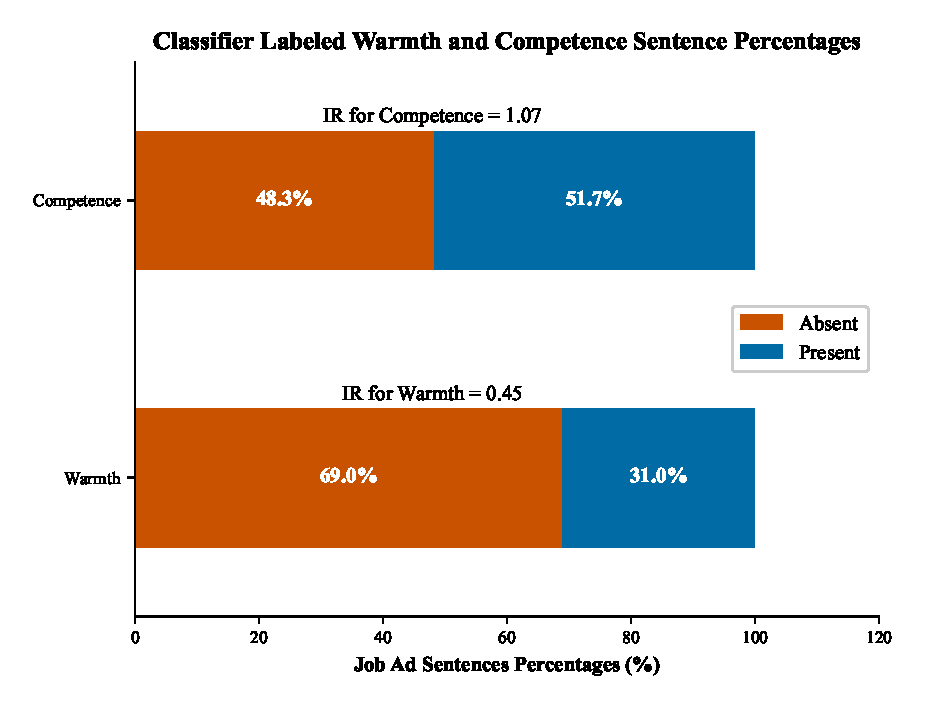
\includegraphics[width=0.95\columnwidth]{ir.eps}
% % \end{figure}

% Hyperparameters optimization was done via Halving Grid Search, a successive halving algorithm that reduces the cost of optimization by exponentially decreasing the number of candidate models at each search iteration while increasing the resources and training cases given to each successful candidate \parencite{soper_hyperparameter_2023}.

% For the transformers, unprocessed data were fed to BERT base uncased \parencite{devlin_bert_2018} and OpenAI GPT2 \parencite{radford2019language} models for sequence classification and their respective fast tokenizers finetuned via HuggingFace’s Trainer class \parencite{wolf_transformers_2020}; train epochs=3, weight decay= 0.01, learning rate=5e-5 (optimized via AdamW). To remedy warmth class imbalance, a customer loss function that corrected imbalance based on class weights was included.

% \subsubsection{Final Model}
% \label{final_model}
% The models were evaluated on the held-out testing and validation sets and selection criteria were based on recall of the positive class, Matthews correlation coefficient (MCC), area-under-the-curve (AUC), and precision-recall curve \parencite{burscher_teaching_2014, chicco_advantages_2020, lever_classification_2016, seliya_study_2009}. Additional considerations included whether a given combination performed better than a baseline dummy classifier and a Naïve Bayes model \parencite{choudhary_comprehensive_2017}. Table~\ref{table:classification_metrics_warmth} and Table~\ref{table:classification_metrics_competence} in \ref{app:A} provide an overview of the models used and their performance metrics.

% For both warmth- and competence-related frame classification, BERT for sequence classification had better overall results on validation; warmth recall =0.81, MCC=0.66, precision=0.72, accuracy=0.86, f1-score=0.76, AUC=0.92; and competence recall=0.86, MCC=0.67, precision=0.80, accuracy=0.83, f1-score=0.83, AUC=0.90.
% The trained model was then used to label job ad sentences as not containing warmth/competence-related frames (0) or containing related to warmth/competence-related frames (1) respectively; warmth \textit{n}\textsubscript{sentences} present=95276 (31.0\%), \textit{n}\textsubscript{sentences} absent=211878 (69.0\%), M=0.31, SD=0.46, and competence \textit{n}\textsubscript{sentences} present=158797 (51.7\%), \textit{n}\textsubscript{sentences} absent=148357 (48.3\%), M=0.52, SD=0.50. Furthermore, the model provided probabilities for the presence of warmth- and competence- in a job ad sentence, which were then used for analysis (see \ref{dv}). Table~\ref{table:k_alpha} shows the distribution of positive and negative classes for warmth- and competence-related sentences (\textit{n}\textsubscript{sentences}=307154) and the classification reports for the selected models. Figure~\ref{fig:warmth_bert_all} to \ref{fig:competence_bert_calibration} in Appendix~\ref{app:A} show the confusion matrices, precision-recall curve, ROC, and calibration curve.

% % \begin{table}[H]
% %     \centering
% %     \caption{Classification report for final model}
% %     \label{table:classification_report}
% %     \centering
% %     \begin{NiceTabular}[tabularnote = {\vspace{0.5pt}\raggedright\footnotesize\item\textit{Note.} “-” indicates values that are not calculated by evaluation modules.}]{@{}L{0.2}C{0.1}C{0.1}C{0.12}C{0.12}C{0.12}C{0.12}}
% %         \toprule
% %         \multirow{2}{*}{Warmth} & \multirow{2}{*}\textit{n}\textsubscript{sentences} & \multirow{1}{*}\% & \multicolumn{4}{c}{BertForSequenceClassification + BertTokenizerFast} \\
% %         \cmidrule{4-7}
% %         ~ & ~ & ~ & Precision & Recall & F1-score & Support \\
% %         \midrule

% %         Not present (0) & 211878 & 69.0\% & 0.92 & 0.88 & 0.90 & 1063 \\
% %         Present (1) & 95276 & 31.0\% & 0.72 & 0.81 & 0.76 & 419 \\
% %         Accuracy & - & - & - & - & 0.86 & 1482 \\
% %         Macro-average & - & - & 0.82 & 0.84 & 0.83 & 1482 \\
% %         Weighted-average & - & - & 0.86 & 0.86 & 0.86 & 1482 \\
% %         \midrule

% %         \multirow{2}{*}{Competence} & \multirow{2}{*}\textit{n}\textsubscript{sentences} & \multirow{1}{*}\% & \multicolumn{4}{c}{BertForSequenceClassification + BertTokenizerFast} \\
% %         \cmidrule{4-7}
% %         ~ & ~ & ~ & Precision & Recall & F1-score & Support \\
% %         \midrule

% %         Not present (0) & 148357 & 48.3\% & 0.87 & 0.81 & 0.84 & 800 \\
% %         Present (1) & 158797 & 51.7\% & 0.80 & 0.86 & 0.83 & 682 \\
% %         Accuracy & - & - & - & - & 0.83 & 1482 \\
% %         Macro-average & - & - & 0.83 & 0.84 & 0.83 & 1482 \\
% %         Weighted-average & - & - & 0.84 & 0.83 & 0.83 & 1482 \\
% %         \bottomrule
% %     \end{NiceTabular}
% % \end{table}

% \subsection{Variables}
% \label{variables}

% \subsubsection{Dependent Variables}
% \label{dvs}
% \paragraph{Probability of Warmth- and Competence-Related Frames Presence in Sentence.}
% \label{dvs_prob}
% The dependent variable examined is the (probability of) presence of warmth- and competence-related frames in job ads sentences as indicated by the extent to which the two concepts are emphasized in text. This variable is measured at a continuous level; warmth \textit{M}=0.31, \textit{SD}=0.38, range=0.004-0.964, and competence \textit{M}=0.47, \textit{SD}=0.38, range=0.004-0.944. We obtained probabilities of predictions from the trained automated classifier, and we use these instead of binary predictions\endnote{To confirm a strong linear relationship between the binary predictions and the probabilities of predictions, we conduction an OLS regression with probabilities as dependent variable and predictions as independent variable; warmth \textit{F}(1, 1481)=22960.00, \textit{p}=.00, \textit{b}=0.86, \textit{t}=151.51, \textit{p}=.00, and competence \textit{F}(1, 1481)=23440.00, \textit{p}=.00, \textit{n}=0.80, \textit{t}=153.11, \textit{p}=.00.}. We argue that the extent of emphasis is variable (vs. binary), thus probabilities provide a more fine-grained measure in addition to allowing for more robust linear modeling and discussion of likelihood.

% % \begin{table}[H]
% %     \centering
% %     \caption{Number and proportions of collected job advertisements, resulting sentences, and descriptive statistics for percentages of gender and age social category composition per sector}
% %     \label{table:dvs_prob}

% %     \begin{NiceTabular}{@{}L{0.2}C{0.07}C{0.07}C{0.12}C{0.07}C{0.07}C{0.07}C{0.12}C{0.07}}
% %         \toprule
% %         \multicolumn{9}{c}{Collected Dataset Job Advertisements} \\
% %         \midrule

% %         \multirow{2}{0.20\columnwidth}{Stereotype \linebreak[3]frames} & \multicolumn{4}{c}{Job Advertisement} & \multicolumn{4}{c}{Sentence} \\
% %         \cmidrule{2-9}
% %         ~ & \textit{M} & \textit{SD} & 95\% Conf. & Interval & \textit{M} & \textit{SD} & 95\% Conf. & Interval \\
% %         \midrule
% %         Warmth Probability & 0.25 & 0.35 & 0.25 & 0.26 & 0.31 & 0.38 & 0.31 & 0.32 \\
% %         Competence Probability & 0.43 & 0.35 & 0.42 & 0.43 & 0.47 & 0.35 & 0.47 & 0.47 \\
% %         \bottomrule

% %     \end{NiceTabular}
% % \end{table}

% \paragraph{Operationalization}.
% \label{dvs_prob_op}
% To operationalize warmth and competence, definitions from Fiske et al. (2002) were supplemented with insights from our codebook construction procedure and relevant research in social psychology and organizational communication \parencite[e.g.,][]{bruckmuller_density_2013, gaucher_evidence_2011, krings_stereotypical_2011, kroon_reliable_2018, van_selm_search_2021}. The operational definition for warmth-related frames centered around whether a sentence highlights people-orientation and features interpersonal and community-building elements. For competence-related frames, the definition relied on whether a sentence highlights task- and outcome-orientation and emphasizes technical and productivity-centric elements (see Codebook~\ref{codebook} in Appendix~\ref{app:A})

% \subsubsection{Independent Variables}
% \label{ivs}
% The independent variable is the categories of sectors as demarcated by respective gender and age segregation. This variable is measured at two levels: (1) continuous percentages of each social category in a given sector, and (2) categorical designations of a given sector.

% \paragraph{Percentages of Social Category per Sector (PPS).}
% \label{ivs_pps}
% On gender, the percentages of female workers per sector range from a minimum of 12.5\% (Construction) to 84.3\% (Health and social work activities); \textit{M}=45.36, \textit{SD}=19.49. For male workers, the range is from 15.6\% (Health and social work activities) to 87.5\% (Construction); \textit{M}=54.60, \textit{SD}=19.52. On age, the percentages of older workers per sector range from a minimum of 18.9\% (Accommodation and food serving) to 58.3\% (Water supply and waste management); \textit{M}=40.86, \textit{SD}=10.12. For younger workers, the range is from 44.4\% (Water supply and waste management) to 80.8\% (Accommodation and food serving); \textit{M}=59.04, \textit{SD}=9.98. Note that this variable does not include sectors mixed in gender and age.

% % \begin{table}[H]
% %     \centering
% %     \caption{Number and proportions of collected job advertisements, resulting sentences, and descriptive statistics for percentages of gender and age social category composition per sector}
% %     \label{table:ivs_pps}

% %     \begin{NiceTabular}[b]{@{}L{0.20}C{0.07}C{0.07}C{0.12}C{0.07}C{0.07}C{0.07}C{0.12}C{0.07}}
% %         \toprule
% %         \multicolumn{9}{c}{Collected Dataset Job Advertisements} \\
% %         \midrule

% %         \multirow{3}{0.20\columnwidth}{Percentages per\linebreak Sector (PPS)} & \multicolumn{8}{c}{Gender Percentages per Sector (\%)} \\
% %         \cmidrule{2-9}
% %         ~ & \multicolumn{4}{c}{Job Advertisement} & \multicolumn{4}{c}{Sentence} \\
% %         \cmidrule{2-9}
% %         ~ & \textit{M} & \textit{SD} & 95\% Conf. & Interval & \textit{M} & \textit{SD} & 95\% Conf. & Interval \\
% %         \midrule

% %         Female & 43.82 & 18.86 & 43.53 & 44.11 & 45.36 & 19.49 & 45.29 & 45.43 \\
% %         Male & 56.13 & 18.89 & 55.84 & 56.42 & 54.60 & 19.52 & 54.53 & 54.66 \\
% %         \midrule

% %         \multirow{3}{0.20\columnwidth}{Percentages  per\linebreak Sector (PPS)} & \multicolumn{8}{c}{Age Percentages per Sector (\%)} \\
% %         \cmidrule{2-9}
% %         ~ & \multicolumn{4}{c}{Job Advertisement} & \multicolumn{4}{c}{Sentence} \\
% %         \cmidrule{2-9}
% %         ~ & \textit{M} & \textit{SD} & 95\% Conf. & Interval & \textit{M} & \textit{SD} & 95\% Conf. & Interval \\
% %         \midrule

% %         Older & 40.61 & 10.23 & 40.45 & 40.76 & 40.86 & 10.12 & 40.83 & 40.90 \\
% %         Younger & 59.26 & 10.14 & 59.10 & 59.41 & 59.04 & 9.98 & 59.00 & 59.07 \\
% %         \bottomrule

% %     \end{NiceTabular}
% % \end{table}

% \paragraph{Categorical Dominant Social Category of Sector.}
% \label{ivs_dummy}
% On gender, sectors were categorized as (1) female-dominated; \textit{n}=78096 (25.4\%), \textit{M}=0.25, \textit{SD}=0.44, (2) male-dominated; \textit{n}=112675 (36.7\%), \textit{M}=0.37, \textit{SD}=0.48, or (3) mixed-gender; \textit{n}=116529 (37.9\%), \textit{M}=0.38, \textit{SD}=0.49. On age, sectors were categorized as (1) older-dominated; \textit{n}\textsubscript{sentences}=62737 (20.4\%), \textit{M}=0.20, \textit{SD}=0.40, (2) younger-dominated; \textit{n}=46937 (15.3\%), \textit{M}=0.15, \textit{SD}=0.36, or (3) mixed-age; \textit{n}=197626 (64.3\%), \textit{M}=0.64, \textit{SD}=0.48. Note that these variables were dummy coded to allow linear analysis.

% % \begin{table}[H]
% %     \centering
% %     \caption{Number and proportions of collected job advertisements, resulting sentences, and descriptive statistics for gender and age dominant social category per sector}
% %     \label{table:ivs_dummy}

% %     \begin{NiceTabular}{@{}L{0.22}C{0.07}C{0.07}C{0.07}C{0.07}C{0.07}C{0.07}C{0.07}C{0.07}}
% %         \toprule
% %         \multicolumn{9}{c}{Collected Dataset Job Advertisements} \\
% %         \midrule

% %         \multirow{3}{*}{Sectors} & \multicolumn{8}{c}{Gender Categorical Designation of Sector} \\
% %         \cmidrule{2-9}
% %         ~ & \multicolumn{4}{c}{Job Advertisement} & \multicolumn{4}{c}{Sentence} \\
% %         \cmidrule{2-9}
% %         ~ & \textit{n} & \% & \textit{M} & \textit{SD} & \textit{n} & \% & \textit{M} & \textit{SD} \\
% %         \midrule

% %         Female-dominated & 3475 & 21.5 & 0.22 & 0.41 & 78092 & 25.4 & 0.25 & 0.44 \\
% %         Mixed Gender & 6301 & 39.1 & 0.39 & 0.49 & 116458 & 37.9 & 0.38 & 0.49 \\
% %         Male-dominated & 6359 & 39.4 & 0.39 & 0.49 & 112604 & 36.7 & 0.37 & 0.48 \\
% %         Total & 16135 & 100.0 &  &  & 307154 & 100.00 &  &  \\
% %         \midrule

% %         \multirow{3}{*}{Sectors} & \multicolumn{8}{c}{Age Categorical Designation of Sector} \\
% %         \cmidrule{2-9}
% %         ~ & \multicolumn{4}{c}{Job Advertisement} & \multicolumn{4}{c}{Sentence} \\
% %         \cmidrule{2-9}
% %         ~ & \textit{n} & \% & \textit{M} & \textit{SD} & \textit{n} & \% & \textit{M} & \textit{SD} \\
% %         \midrule

% %         Older-dominated & 3605 & 22.3 & 0.22 & 0.42 & 62705 & 20.4 & 0.20 & 0.40 \\
% %         Mixed Gender & 10277 & 63.7 & 0.64 & 0.48 & 197512 & 64.3 & 0.64 & 0.48 \\
% %         Younger-dominated & 2253 & 14.0 & 0.14 & 0.35 & 46937 & 15.3 & 0.15 & 0.36 \\
% %         Total & 16135 & 100.0 &  &  & 307154 & 100.0 &  &  \\
% %         \bottomrule

% %     \end{NiceTabular}
% % \end{table}

% \paragraph{Categorical Operationalization.}
% \label{ivs_dummy_op}
% To arrive at a discrete categorical classification, an approach advocated by \Textcite{hakim_segregated_1993} was utilized where a threshold is set in order to demarcate segregated and non-segregated occupational domains, including at the sectoral level. This approach has been employed by researchers examining horizontal occupational segregation from sociological perspectives \parencite[e.g.,][]{jacobs_theoretical_1993, van_der_lippe_comparative_2002} and is further utilized by the European Commission’s Expert Group on Gender and Employment \parencite[EGGE;][]{bettio2009GenderSegregationLabour}. Unlike other occupational segregation measures where a score indicates the level of segregation over the entire cross-national workforce, the index proposed by Hakim allows computing segregated sectors into discrete categories. Note that the threshold for demarcating older- vs. younger-dominated sectors is at 45 years of age given that employers assess candidates’ age relative to other candidates as well as other workers within a sector \parencite{van_selm_search_2021}.

% In practice, the approach entails setting a threshold in the form of a percentage-point spread around the overall proportion of a selected reference group employed in the workforce. For example, if a threshold is set at 10\% for a workforce where the reference group comprises 40\% of all workers, then a sector with 30\% reference group members or less (40\% - 10\%) is classified as not dominated by the reference group and a sector with 50\% reference group members or more (40\% + 10\%) is classified as dominated by the reference group.

% In 2020, the Dutch workforce comprised 47.6\% female workers, 52.4\% male workers, 42.1\% workers aged 45 and over, and 57.9\% workers below the age of 45 \parencite{centraal_bureau_voor_de_statistiek_sustainable_2019, oecd2020OECDLabourForce}. The reference group for categorizing sector segregation by gender is females, and for age, older workers were referenced. Following the ratios used by \Textcite{hakim_segregated_1993} and \Textcite{bettio2009GenderSegregationLabour}, a threshold of 15\% demarcated sector segregation by gender and 10\% demarcated sector segregation by age. For gender, sectors were classified as male-dominated if they comprise 32.6\% women or less, and female-dominated if they comprise 62.6\% women or more. For age segregation, sectors were classified as younger-dominated if they comprise 32.1\% older workers or less, and older-dominated if they comprise 52.1\% older workers or more. Sectors that did not fall within these thresholds were classified as mixed in gender and age respectively. Table~\ref{table:cbs_keywords} to Table~\ref{table:cbs_age} in Appendix~\ref{app:A} shows the composition and age- and gender-dominance categorization of sectors and Table~\ref{table:ivs_dummy} show the sample sizes and distribution of job ads across sectors.

% \subsubsection{Control Variables}
% \label{controls}
% \paragraph{Sector Percentage per Workforce (PPW).}
% \label{ppw}
% This variable is measured at a continuous ratio level and denotes the share of a given sector from the total workforce; \textit{M}=5.42, \textit{SD}=8.77. The sector Energy supply had the lowest workforce share (0.1\%), and Commercial services had the highest (31.4\%). Controlling for this covariate attenuates the effects of larger sectors on the analysis model.

% \paragraph{Number of Words per Sentence.}
% \label{num_words}
% This variable is measured at a continuous interval level and is a count of the number of words (excluding non-alphanumeric characters) per sentence; range=3-349, \textit{M}=17.67, \textit{SD}=16.45. Controlling for this covariate attenuates the effects of shorter sentences on the analysis model.

% \subsubsection{Analysis Method}
% \label{analysis}
% To test our hypotheses, we employ Specification Curve Analysis (SCA), a frequentist analysis technique that “… consists of reporting the results for all (or a large random subset thereof) ‘reasonable specifications” \parencite[1208]{simonsohn_specification_2020}. Specifications here refer to all combinations of model variables (independent, dependent, and control) that are theoretically relevant, statistically valid, and non-redundant. Further, variables with differing operationalization and/or measurement can be included simultaneously \parencite[see][]{frey_identifying_2020}.

% Given that the measurements of our independent variable not only correlate with each other but also among each other (viz., high correlation between homogeneous and heterogeneous sector categories, Figure~\ref{fig:correlations}), a single model could not account for all predictors without sacrificing robustness. The SCA is suited for the current study as it reveals whether results as a whole are (in)consistent with the null hypothesis \parencite{simonsohn_specification_2015}. The SCA has additionally been found to attenuate the effects of arbitrary research decisions \parencite[i.e., researchers’ degrees of freedom, see][]{babyak_what_2004}, reduce selective analysis and reporting \parencite{huang_beyond_2022}, increase transparency \parencite{jussim_research_2022}, and facilitate intuitive reading and understanding of the results. For a practical guide to SCA, see \Textcite{cosme_specification_2020}. Examples of academic use of SCA are present in fields of psychology \parencite{frey_identifying_2020, rauvola_worker_2023, twenge_specification_2022}, human behavior \parencite{orben_association_2019}, and communication studies \parencite{masur_understanding_2023}.

% The method entails performing numerous regression analyses on different specifications and the results are displayed in graphic format. The specification curve within the specification panel shows color-coded unstandardized coefficients of all the tested regression models along with their confidence intervals (error bars) indicating model significance. A gray error bar indicates a non-significant model whereas a blue or red error bar indicates significance. A red error bar indicates a negative coefficient whereas a blue bar indicates a positive one. All included variables are listed at the bottom of the panel. Information about a single model is read vertically. A dash in a variable’s row, i.e., a decision, indicates the variable was included in the model that gave the coefficient aligned directly above the dash. Singular regression models can also be retrieved and reported.

% For linear analysis, we assessed multicollinearity by examining the correlations and VIF scores of the control variables and the dummy-coded categorical designations of sectors (Appendix~\ref{app:A}, \ref{fig:correlations}). A very high correlation was found between all independent variables; range=1.00- 347540195807.42. Removing homogeneous sector categories improved VIF scores to an acceptable level; range=1.00-2.26. Control variables separately also showed acceptable VIF scores; range=1.00-1.00. Note that the multicollinearity test did not include the PPS variables as those naturally correlate with the dummy coded homogeneous sectors variables as well as each other. In total, 14 variables were used for each SCA model resulting in 40 specifications.

% We performed SCA via the Python library provided by \Textcite{aeturrell_2022_7264033} and used OLS regression with continuous probabilities of warmth and competence predictions regressed on both continuous percentages of social category per sector and dummy-coded categorical designations of sectors as independent variables. The SCA provides results for single regressions between each dependent and independent variable, so we additionally conducted a multiple regression analysis that includes all variables for comparison.

% \subsection{Results}
% \label{results}
% The SCA panel (Figure~\ref{fig:sca}) shows that overall, the presence of warmth- and competence-related frames vary widely among sectors, and competence-related frames were naturally more observed; warmth \textit{R}\textsuperscript{2} range=0.126-0.129, RMSE range=0.350-0.351, \textit{F}\textsubscript{Full}(10, 307154)=4584.83, \textit{p}\textsubscript{Full}=0.00, \textit{R}\textsuperscript{2}\textsubscript{Full}=0.13, and competence \textit{R}\textsuperscript{2} range=0.113-0.115, RMSE range=0.329-0.329, \textit{F}\textsubscript{Full}(10, 307154)=4102.11, \textit{p}\textsubscript{Full}=0.00, \textit{R}\textsuperscript{2}\textsubscript{Full}=0.12. There is a significant positive association between the presence of warmth-related frames in job ads and female-typed sectors as well as a significant positive association between the presence of competence-related frames and male-typed sectors. We also note a negative association between the presence of competence-related frames and female-typed sectors and the presence of warmth-related frames and male-typed sectors.

% The findings thus far are in line with our expectations, however, the SCA shows that results are inconsistent with our hypotheses regarding age-typed sectors and the presence of warmth- and competence-related frames. Younger-typed sectors are not only positively associated with the presence of warmth-related frames, but there is also a noticeable negative association with the presence of competence-related frames. Strikingly, older-typed sectors are negatively associated with the presence of warmth-related frames and show a strong positive association with the presence of competence-related frames – the strongest association in the SCA curve. We explore these associations further and examine the regression models. Table~\ref{table:sca_warmth} and Table~\ref{table:sca_competence} in Appendix~\ref{app:A} show all SCA regression statistics including the multiple regression analysis. Note that we report only models that include all control variables.

% % \begin{figure}
% %     \caption{OLS regression-based Specification curve}
% %     \label{fig:sca}
% %     \centering
% %     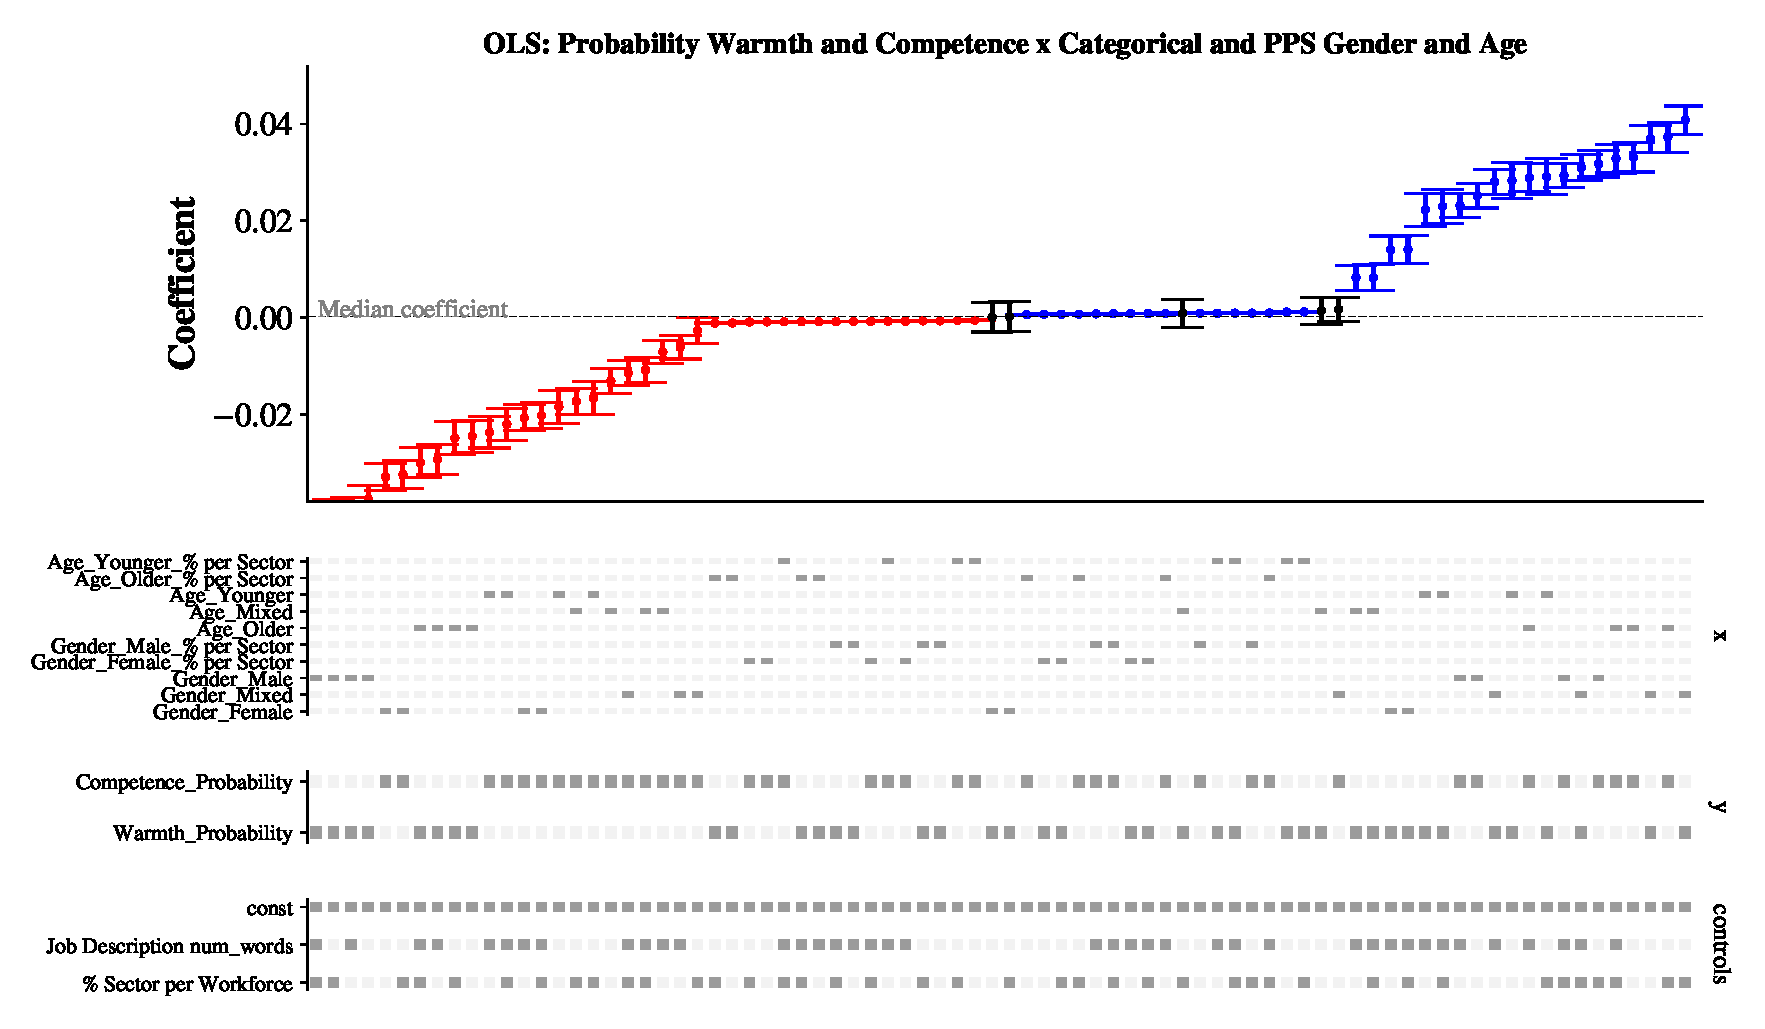
\includegraphics[width=\columnwidth]{sca.eps}
% %     \raggedright\fnote{
% %         \item\footnotesize\itshape{
% %         Note.
% %         \linebreak
% %         Dependent variable: Probability of Warmth- and Competence-Related Frames Presence in Sentence
% %         \linebreak
% %         Independent variables: (1) Categorical Dominant Social Category of Sector and (2) Percentages of Social Category per Sector
% %         \linebreak
% %         Control variables: (1) Sector Percentage per Workforce and (2) Number of Words per Sentence}
% %         }
% % \end{figure}

% We first examine the hypotheses regarding the relationship between sectoral gender segregation and the presence of stereotypical frames in job ads. Hypothesis H1a states that job ads from female-dominated sectors will contain significantly more warmth-related frames when compared to ads from male-dominated sectors and H1b states that job ads from female-dominated sectors will contain significantly more warmth-related frames compared to ads from mixed-gender sectors. Job ads from female-dominated sectors; \textit{\textbeta}=0.032, \textit{t}=9.69, \textit{p}=.00, \textit{M}=0.32, \textit{SD}=0.38, and those with higher percentages of female workers; \textit{\textbeta}=0.0000, \textit{t}=25.76, \textit{p}=.00, were more likely to contain warmth-related frames compared to jobs ads from male-dominated sectors; \textit{\textbeta}=-0.090, \textit{t}=-31.39, \textit{p}=.00, \textit{M}=0.29, \textit{SD}=0.37, and those with higher percentages of male workers; \textit{\textbeta}=-0.0000, \textit{t}=-25.82, \textit{p}=.00, thus H1a is supported. Conversely, job ad sentences from female-dominated sectors were less likely to contain warmth-related frames compared to job ad sentences from mixed-gender sectors; \textit{\textbeta}=0.064, \textit{t}=22.34, \textit{p}=.00, \textit{M}=0.34, \textit{SD}=0.38, thus H1b is rejected.

% Hypothesis H2a states that job ads from male-dominated sectors will contain significantly more competence-related frames when compared to ads from female-dominated sectors and H1b states that job ads from male-dominated sectors will contain significantly more competence-related frames compared to ads from mixed-gender sectors. Job ad sentences from male-dominated sectors; \textit{\textbeta}=0.061, \textit{t}=22.74, \textit{p}=.00, \textit{M}=0.49, \textit{SD}=0.35, and those with higher percentages of male workers; \textit{\textbeta}=0.0000, \textit{t}=25.83, \textit{p}=.00, were more likely to contain competence-related frames compared to jobs ads from female-dominated sectors; \textit{\textbeta}=-0.046, \textit{t}=-14.79, \textit{p}=.00, \textit{M}=0.45, \textit{SD}=0.35, and those with higher percentages of female workers; \textit{\textbeta}=-0.0000, \textit{t}=-25.73, \textit{p}=.00, thus H2a is supported. Job ad sentences from male-dominated sectors were more likely to contain competence-related frames compared to job ad sentences from mixed-gender sectors; \textit{\textbeta}=-0.024, \textit{t}=-8.79, \textit{p}=.00, \textit{M}=0.47, \textit{SD}=0.35, thus H2b is supported.

% % \begin{figure}
% %     \caption{Classifier labeled dataset line and violin plots of warmth and competence probability distribution across categorical dominant social category of sector}
% %     \label{fig:df_jobs_anova}
% %     \centering
% %     \begin{subfigure}
% %         \centering
% %         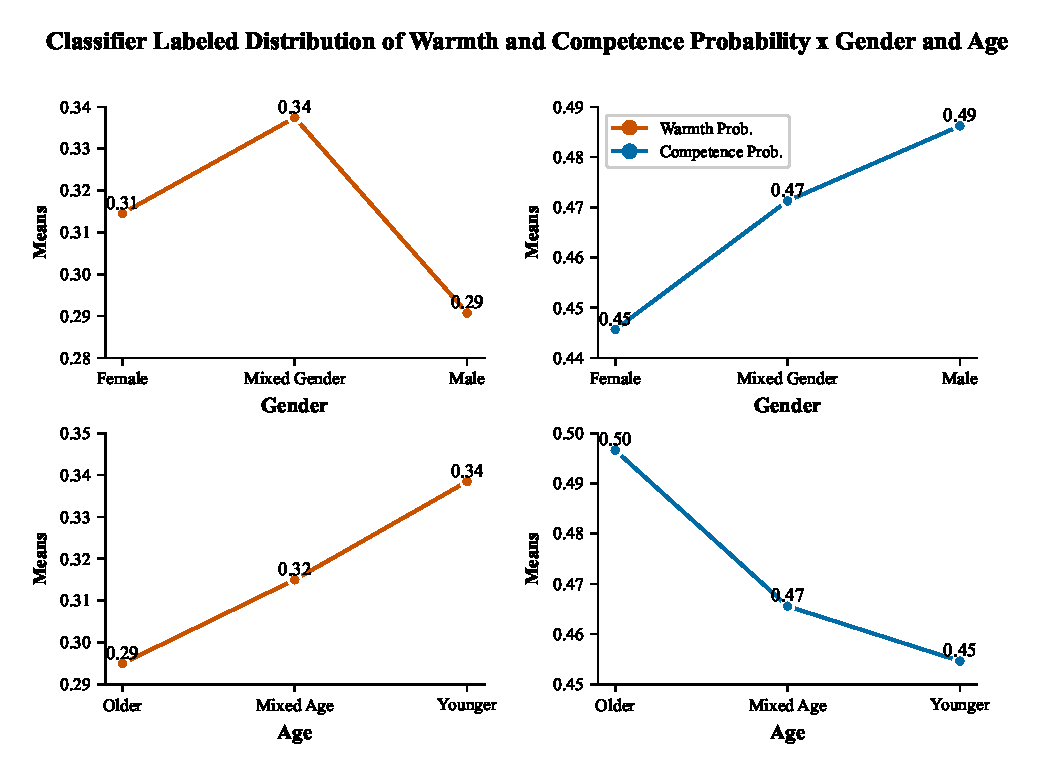
\includegraphics[width=0.50\columnwidth]{df_jobs_lineplot.eps}
% %     \end{subfigure}%
% %     \hfill
% %     \begin{subfigure}
% %         \centering
% %         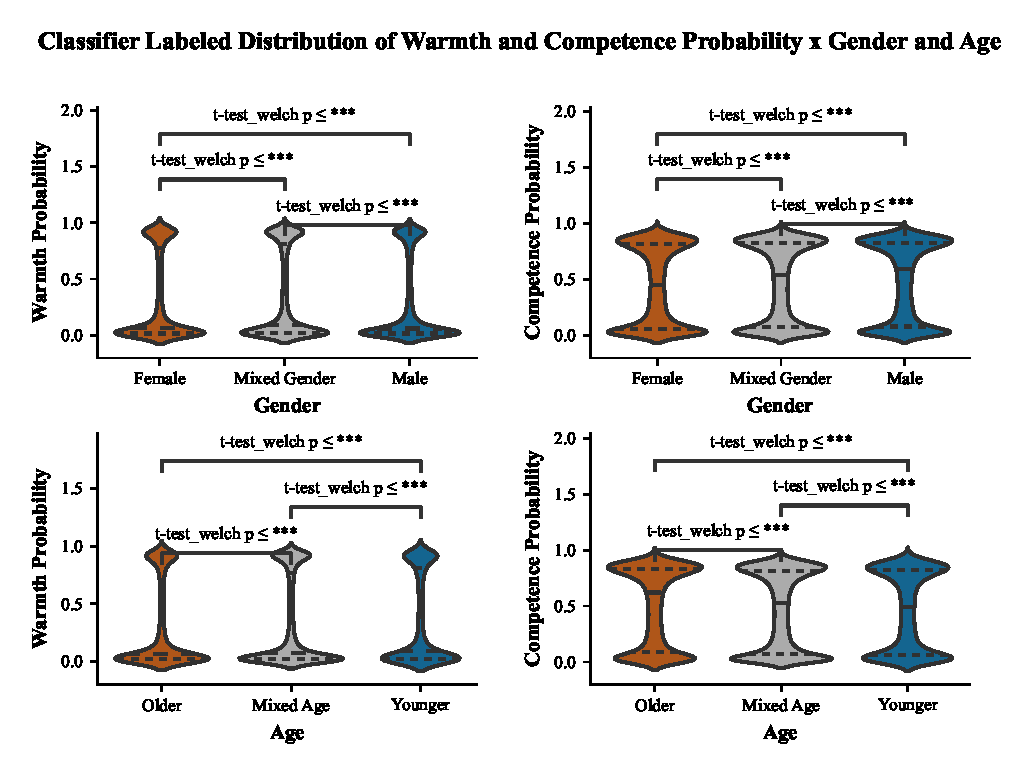
\includegraphics[width=0.50\columnwidth]{df_jobs_violinplot.eps}
% %     \end{subfigure}
% %     \raggedright\fnote{
% %         \item\footnotesize\textit{Note. *\textit{p} < .05 **\textit{p} < .01 ***\textit{p} < .0001}
% %     }
% % \end{figure}

% We now turn to the hypotheses examining the relationship between sectoral age segregation and the presence of stereotypical frames in job ads. Hypothesis H3a states that job ads from older-dominated sectors will contain significantly more warmth-related frames when compared to ads from younger-dominated sectors and H3b likewise states that job ads from older-dominated sectors will contain significantly more warmth-related frames compared to ads from mixed-age sectors. Job ad sentences from older-dominated sectors; \textit{\textbeta}=-0.074, \textit{t}=-18.75, \textit{p}=.00, \textit{M}=0.29, \textit{SD}=0.37, and those with higher percentages of older workers; \textit{\textbeta}=-0.0001, \textit{t}=-13.59, \textit{p}=.00, are less likely to contain warmth-related frames compared to jobs ads from younger-dominated sectors; \textit{\textbeta}=0.064, \textit{t}=12.95, \textit{p}=.00, \textit{M}=0.34, \textit{SD}=0.38, and those with higher percentages of younger workers; \textit{\textbeta}=0.0001, \textit{t}=14.19, \textit{p}=.00, thus we reject H3a. Job ad sentences from older-dominated sectors were less likely to contain warmth-related frames compared to job ad sentences from mixed-age sectors; \textit{\textbeta}=0.017, \textit{t}=6.04, \textit{p}=.00, \textit{M}=0.32, \textit{SD}=0.38, thus H3b is rejected.

% Hypothesis H4a states that job ads from younger-dominated sectors will contain significantly more competence-related frames when compared to ads from older-dominated sectors and H4b likewise states that job ads from younger-dominated sectors will contain significantly more competence-related frames compared to ads from mixed-gender sectors. Job ad sentences from younger-dominated sectors; \textit{\textbeta}=-0.061, \textit{t}=-13.26, \textit{p}=.00, \textit{M}=0.46, \textit{SD}=0.35, and those with higher percentages of younger workers; \textit{\textbeta}=--0.0001, \textit{t}=-14.47, \textit{p}=.00, are less likely to contain competence-related frames compared to jobs ads from older-dominated sectors; \textit{\textbeta}=0.081, \textit{t}=21.87, \textit{p}=.00, \textit{M}=0.50, \textit{SD}=0.35, and those with higher percentages of older workers; \textit{\textbeta}=0.0001, \textit{t}=15.96, \textit{p}=.00, thus H4a is rejected. Job ad sentences from younger-dominated sectors were less likely to contain competence-related frames compared to job ad sentences from mixed-age sectors; \textit{\textbeta}=-0.023, \textit{t}=-8.46, \textit{p}=.00, \textit{M}=0.47, \textit{SD}=0.35, thus H3b is rejected.

% \section{Discussion}
% \label{discussion}
% In conducting this study, we set out to examine the stereotypical frames present in job advertisements as indicated by the differential emphasis on warmth and competence characteristics, and to empirically investigate the link between the presence of such frames and macro-level, i.e., sectoral, occupation gender and age segregation. We put forth an operationalization of broad-level gender- and age-related stereotypical frames that are compatible with the axioms of the stereotype content model (SCM) and adapted specifically to examine early candidate sourcing communication. As per the operationalization presented, warmth in the occupational domain is communicated by emphasizing an orientation towards people, team and community building, and strong interpersonal characteristics. Occupational competence, conversely, is conveyed by emphasizing productivity, performance on tasks, measurable outcomes, and the display of technical acumen.

% With regards to the relationship between the gender-stereotypical framing of job ads and sectoral segregation, our findings show that job ads from female-dominated sectors tend to emphasize warmth but do not differ from mixed-gender sectors on this dimension. Conversely, ads from male-dominated sectors tend to emphasize competence and de-emphasize warmth. This indicates that differences stem chiefly from the framing of ads from male-dominated sectors. The emphasis on competence in job ads from male-dominated sectors but not in ads from female-dominated align with social categorization framing. This framing signals social category-based ownership of segregated sectors and suggests some endorsement of traditional gender essentialism particularly as it pertains to work and gendered perceptions of competence. These findings support the egalitarian gender essentialism paradigm suggested by \Textcite{cotter_end_2011} to explain the gender-equality paradox observed in liberal egalitarian societies such as the Netherlands.

% With regards to the correlation between age-stereotypical job ads framing and sectoral segregation, our findings show an opposite effect to our expectations regarding warmth-related frames among age homogeneous and heterogeneous sectors. Ads from older-dominated sectors were significantly more likely to contain competence-related frames compared to ads from younger-dominated and mixed-age sectors. Job ads from younger-dominated sectors also contained significantly more warmth-related frames compared to mixed-age sectors.

% These results are not in line with studies about older individuals, however, age-related warmth stereotypes may not be as readily transferable to the context of hiring and recruitment communication despite older individuals being stereotyped as warm. Findings from \Textcite{abrams_old_2016} and \Textcite{krings_stereotypical_2011} show that warmth characteristics are consistently linked to older workers, however, a requirement of warmth characteristics in an offered position did not predict targeting towards or a preference for older job seekers. Furthermore, \Textcite{krings_stereotypical_2011} also found that when explicitly evaluating candidates for hiring as opposed to a context-free evaluation, older job seekers were perceived as less warm than their younger counterparts. Thus, older individuals may be perceived as warm whereas older workers may demonstrate qualities such as experience, knowledge-sharing motivations, or rich social capital that counteract stereotypical age perceptions.

% Markedly, the strength of the association shows that there exists sectoral “ownership” and respective social category framing, although, in a direction opposite to what was expected. In the long run, this association may prove beneficial to older workers as the workforce age has increased over the past decades \parencite{oude_mulders_how_2020-1} and will continue this trend with increased retirement age pension reform in the Netherlands particularly \parencite{pilipiec_analysis_2022} and Europe generally \parencite{axelrad_actual_2022}.

% The significant positive relationship between younger-dominated sectors and the presence of warmth-related frames is possibly a reflection and consequence of changing attitudes among younger people towards work. Younger workers value open communication, show a desire for learning, are team-oriented, and prioritize the social aspect of their jobs \parencite{baker_rosa_managing_2018, myers_millennials_2010}. These attitudes being reproduced in job ads targeting younger workers may be a sign that candidate sourcing practices are more in tune with the evolving workplace and undergoing adaption.

% Nevertheless, our findings on the presence of warmth-related frames in job ads from female-dominated sectors suggest more research is needed to explain this disparity between gender-based and age-based warmth stereotypes. Researchers may benefit from exploring confounding factors such as differences in value ascribed to warmth characteristics during hiring, valence of stereotype content \parencite{suitner_role_2008}, or perceptions of older workers in a given context \parencite{hennekam_employability_2015}.

% \subsection{Societal Implications}
% \label{implications}
% Tentatively, the findings presented indicate partial support for social categorization framing in candidate sourcing and its exercise in employer communication addressing different gender and age groups. The differences in warmth- and competence-related frames favor homogeneous sectors, with heterogeneous sectors mostly falling midway. This indicates an emphasis on stereotypical characteristics in these sectors that is not readily transferable (from day-to-day consensual stereotypes) or apparent, but is nonetheless present.
% These results could prove consequential in the context of automated candidate sourcing as more HR processes move to online spaces. Online job search platforms have en-mass developed and deployed various content-based recommender systems (CBR). The predictive algorithms behind these e-Recruitment tools leverage textual features of job ads to target job seekers \parencite{pejic-bach_text_2020, shi2020SalienceMarketawareSkill}. With the current advancements in natural language processing, the novel large language models-based (LLM) implementations of CBR systems are able to detect subtle textual indicators of bias and inadvertently perpetuate or even amplify inequitable candidate sourcing \parencite{singhal_use_2017}. The small differences found in the present study may be amplified when considering the large corpus required to train hiring algorithms. Amazon, for instance, discontinued its machine learning-based recruitment tool after the algorithms learned to downgrade or even exclude resumes that contained terms like ‘women’s chess club’ or names of all-womens’ colleges \parencite{dastin2018AmazonScrapsSecret}. Although this example may be an excess within the larger context of automated hiring and recruitment, it does show the potential impact of these approaches if not addressed. The results of this study thus provide empirical foundation for examining stereotypical frames in job ads as automation becomes the norm in candidate sourcing.

% Beyond consequences for candidate sourcing, the presence of stereotypical frames in early employer communication has consequences for job seekers who are exposed to these messages. According to \Textcite{Yang2015a}, the significant emphasis on dominant social category characteristics serves to makes salient the self-to-others social distance, consequently activating social category stereotyping directed towards outgroups members as well as the self \parencite{Steele1997}. Particular to employer communication, studies indicate usage of such communication, although may initially help target sourcing efforts, ultimately narrows the pool of job seekers who feel addressed by employers’ communication and feel appealed to apply \parencite{zhu_understanding_2021}. Exposure to such communication can have substantial consequences for potential candidates’ perceived social belonging, stereotype threat perceptions, and the level of trust candidates have towards professional settings \parencite{purdie-vaughns_social_2008, walton_question_2007}. Emphasis on stereotypical aspects of a position can also lead job seekers to self-select or self-eliminate based on perceived role incongruity, further narrowing the pool of potential candidates and ultimately decreasing workplace diversity \parencite{henningsen_where_2021}.

% \subsection{Limitations}
% \label{limitations}
% As with any endeavor, this study has some limitations of note. The differences in job ad framing, although exhibiting small effect sizes, are meaningful in the context of the larger media studies paradigm \parencite{Perloff2013}. Regarding sector categorization, we measured occupational segregation via an index devised by \parencite{hakim_segregated_1993} deemed suitable for various reasons including its consideration for part-time workers and its categorical level of measurement. However, we found that the threshold set at 45 years of age following recommendations from extant literature was not conducive to our study when the reference group was older workers as it did not align with normative views on age. We advised future researchers to be cognizant of this and utilize measures of occupational segregation developed with a specific reference social group in mind.

% Regarding the usage of concepts related to warmth and competence in job ads, we find that some qualities cannot be neatly categorized. For instance, concepts related to global or multicultural organizational aspects had to be singled out and described separately in our operationalization (see Codebook~\ref{codebook}) On one hand, emphasis on these aspects could convey an inclusive and diverse workplace, which coders perceived as emphasizing warmth. On the other, many job ads used these aspects to indicate global market presence, which to coders highlighted an organization’s competence. In line with many items we encountered, emphasizing an organization’s multiculturalism seemed to serve both purposes simultaneously, consequently the concept could not be categorized as definitively as preferred. Future researchers are invited to explore offshoots of the SCM, for example, the SCM facet model Agency-Communion-Inventory \parencite[AC-IN;][]{abele_facets_2016}, which distinguish dimensions through motivations, abilities, and similar cognitive mechanisms. We contend that approaching warmth and competence dimensions through their underlying drivers may help delineate concepts in text and constrain their operationalization to factors pertinent to the topic under study.

% References
\printbibliography

\end{document}
